\documentclass[aspectratio=43]{beamer}
% Theme works only with a 4:3 aspect ratio
\usetheme{CSCS}

\usepackage{tikz}
\usepackage{pgfplots}
\usepackage{pgfplotstable}
\usetikzlibrary{pgfplots.groupplots,spy,patterns}
\usetikzlibrary{arrows.meta}
\usetikzlibrary{positioning}
\usepackage{listings}
\usepackage{color}
\usepackage{tcolorbox}
\usepackage{anyfontsize}
\usepackage{xspace}
\usepackage{graphicx}
\usepackage{pifont}

% define footer text
\newcommand{\footlinetext}{Performance-portability: Arbor}

% Select the image for the title page
\newcommand{\picturetitle}{cscs_images/image5.pdf}

% fonts for maths
\usefonttheme{professionalfonts}
\usefonttheme{serif}

% source code listing
\newcommand\TS{\rule{0pt}{2.6ex}}       % Top strut
\newcommand\BS{\rule[-1.2ex]{0pt}{0pt}} % Bottom strut
\newcommand{\hl}[1]{\textbf{\textcolor{blue}{#1}}} % for hilighting optimal entries in tables
\newcommand{\rl}[1]{\textbf{\textcolor{red}{#1}}} % for hilighting sub-optimal entries in tables
\newcommand{\img}[1]{{\Large \textbf{IMAGE {#1}}}}
\newcommand{\hilight}[1]{\textcolor{blue!20!orange}{#1}}
\newcommand{\arbor}{{\ttfamily Arbor}\xspace}
\newcommand{\neuron}{{\ttfamily NEURON}\xspace}
\newcommand{\coreneuron}{{\ttfamily CoreNeuron}\xspace}
\newcommand{\daintmc}[0]{Daint-mc\xspace}
\newcommand{\daintgpu}[0]{Daint-gpu\xspace}
\newcommand{\tave}[0]{Tave-knl\xspace}
\newcommand{\pder}[2]{\frac{\partial{#1}}{\partial{#2}}}

% set indent to a more reasonable level (so that itemize can be used in columns)
\setlength{\leftmargini}{20pt}

\DeclareTextFontCommand{\emph}{\color{blue!85!black}}

\author{\textbf{Ben Cumming}, Nora Abi Akar, Stuart Yates, Thorsten Hater, Anne K\"usters, Alexander Peyser.}
\title{Portable simulation with \arbor.}
\subtitle{CNS*2020}
%\subtitle{CNS*2020 Workshop \emph{Tools and resources for developing and sharing models in computational neuroscience} \date{} }

\begin{document}

% TITLE SLIDE
\cscstitle

%-------------------------------------------
%\begin{frame}[fragile]{Overview}
%   Big Arbor logo

%   Overview of talk
%   \begin{enumerate}
%       \item What is \arbor and its motivation
%       \item Portability (performance)
%       \item Portability (model descriptions)
%       \item Allen model
%   \end{enumerate}
%end{frame}
%-------------------------------------------

%-------------------------------------------
\begin{frame}[fragile]{HPC Requires Portability}
    HPC is required to meet ambitious modeling aims.
    \\ \vspace{15pt}
    All major HPC systems coming online in the next few years will be GPU based:
    \begin{itemize}
        \item Piz Daint @ CSCS (since 2015);
        \item Marconi100 @ Cineca (May 2020);
        \item EuroHPC pre-exascale systems (late 2021);
        \item US ECP pre-exascale and exascale systems (2021-2023)
    \end{itemize}
    \vspace{15pt}
    Tools and models they consume will have to be portable.
\end{frame}
%-------------------------------------------


%-------------------------------------------
\begin{frame}[fragile]{\arbor}
%-------------------------------------------
    \arbor is library for simulation of morphologically-detailed cells in large networks on HPC systems.
    \begin{itemize}
        \item \emph{key aim}: enabling simulation on all HPC systems.
        \item \emph{key aim}: provide rich interface enabling diverse use cases.
    \end{itemize}

    \vspace{10pt}
    \emph{All features} are implemented and optimised on \emph{all platforms}
    \begin{itemize}
        \item All GPUs (CUDA, HIP, Clang-CUDA)
        \item SIMD CPU backends: (AVX, AVX2, AVX512, Neon, SVE).
        \item Distributed simulation (MPI).
    \end{itemize}
    \vspace{10pt}
    This talk will focus on how \arbor facilitates \emph{model portability}.

    %Requires a \emph{rich interface} for defining models.
    %\begin{itemize}
    %    \item Simulation of electrical current in arbitrarily complex morphologies.
    %    \item Arbitrary ion channel and synapse models.
    %    \item Inter-cell communication via spikes on arbitrary networks.
    %\end{itemize}
\end{frame}
%-------------------------------------------

%-------------------------------------------
\begin{frame}[fragile]{Models are varied and complicated}
% I like to use this classic image of a Purkinje cell to illustrate the challenges of
% developing a simulation tool like NEURON, CoreNEURON or Arbor.
% The comp. neuroscience community requires simulation tools that can efficiently simulate
% the different ways to represent this cell:
%       - as a leaky integrate and fire point neuron
%       - as a point neuron with user-supplied coupled odes describing state (e.g. HH)
%       - with few compartments and simple dynamics
%       - with detailed descriptions of every last branch in the arbor with spatial
%         variation between of ion channel distributions and stochastic synapses.
% Users also want the same flexibility in describing network dynamices, gap junctions,
% what variables to record for later analysis and so on.

    \begin{center}
        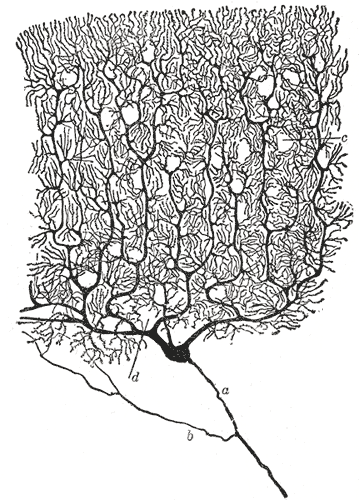
\includegraphics[width=0.45\textwidth]{images/purkinje_cell.png}
        \\
        {
            \scriptsize Drawing of a Purkinje cell in the cerebellar cortex by Santiago Ram\`{o}n y Caja.
        }
    \end{center}
\end{frame}
%-------------------------------------------

%-------------------------------------------
\begin{frame}[fragile]{\arbor}
% Key realisation: developing the efficient hardware optimised implementations of each
% of these model features is quite difficult. *HOWEVER* developing an interface that
% facilitates flexible description of models that can run on those back ends is much
% much harder, and must be integrated correctly with the underlying simulation engine.
%
% Currently, there is one tool that is widely used for this type of simulation: NEURON.
% The reason it stands alone is because it has an interface that allows users to
% describe these diverse models: Arbor does the same.

%    \vspace{30pt}

    The main challenge developing \arbor has been defining an interface for inputing models.
\end{frame}
%-------------------------------------------

%-------------------------------------------
%\begin{frame}[fragile]{\arbor}
%    It is hard to develop a portable tool that provides features and runs efficiently on the platforms we care about:
%    \begin{itemize}
%        \item design work for UI is hard and time consuming
%        \item proper sep. concerns in APIs hard
%        \item low level optimization hard
%    \end{itemize}
%
%    We have spent 5 years working on this problem
%    \begin{itemize}
%        \item one of the biggest challenges with writing a new tool that consumes complex models is model descriptions.
%        \item today I summarise some observations
%    \end{itemize}
%\end{frame}
%-------------------------------------------

%-------------------------------------------
\begin{frame}[fragile]{What is portability, anyway?}
% The challenge really boils down to what I call "portability"
Portability has two aspects:

\begin{enumerate}
\item \emph{Performance portability}, tools that:
    \begin{itemize}
        \item run efficiently and scale on different architectures;
        %\item provide scale-agnostic, reproducable results;
        \item can be adapted to support new architectures.
    \end{itemize}

    \item \emph{Model portability}, model descriptions that are:
    \begin{itemize}
        \item simulator and architecture agnostic;
        \item \emph{flat}, which means:
        \begin{itemize}
            \item what, not how.
            \item translated, not interpreted.
        \end{itemize}
        %\item unambiguous.
    \end{itemize}
\end{enumerate}

\end{frame}

\begin{frame}[fragile]{Facilitating portability in tools}

These concerns are not orthogonal.
\begin{itemize}
    \item Require \emph{separation of concerns} between model description and their implemention.
\end{itemize}

\vspace{10pt}

%Practically, this requires that model descriptions \emph{minimise}:
%\begin{itemize}
    %\item Architecture-specific or simulator-specific information;
    %\item Arbitrary code (Python, HOC, SLI).
%\end{itemize}

Simulation tools can support portable descriptions by:
\begin{enumerate}
    \item Separating hardware and implementation details from model description interface;
    \item Using flat model descriptions in their interface.
\end{enumerate}

\vspace{10pt}

I will now illustrate each of these in \arbor's interface.

\end{frame}

\cscschapter{1. Separate model from implementation.}

% In this next section we will see how Arbor's API enforces this separation between
% model description and the target architecture on which the code will run.
%-------------------------------------------
\begin{frame}[fragile]{Step 1: Model abstraction (which model)}
    User models are described by a \emph{recipe}, which map cell \emph{gid} to:
    \begin{itemize}
        \item a description of the cell
        \begin{itemize}
            \item piecewise linear morphology
            \item named regions and locations
            \item ion channel and synapses
        \end{itemize}
        \item spike targets
        \item spike sources
        \item network connections that terminate on the cell
    \end{itemize}
    \vspace{5pt}
    Recipes provide a consistent flat description for all models.

    \vspace{5pt}
    Recipe descriptions are functional, enabling lazy evaluation for efficient parallel model construction.

    \vspace{5pt}
    Recipes contain no hardware or implementation details.
\end{frame}
%-------------------------------------------

%-------------------------------------------
\begin{frame}[fragile]{Step 2: Hardware context (which hardware)}

        \begin{lstlisting}[style=talkpython]
import arbor
from mpi4py import MPI

rec = my_recipe() # user defined model
ctx = arbor.context(threads=8, gpu_id=0, mpi=MPI.COMM_WORLD)
        \end{lstlisting}


    Users can select hardware resources at run time:
    \begin{itemize}
        \item Number of threads in thread pool
        \item Which GPU [optional]
        \item Which MPI communicator [optional]
    \end{itemize}
\end{frame}
%-------------------------------------------

%-------------------------------------------
\begin{frame}[fragile]{Step 3: Domain decomposition}
        \begin{lstlisting}[style=talkpython]
import arbor
from mpi4py import MPI

rec = my_recipe() # user defined model
ctx = arbor.context(threads=8, gpu_id=0, mpi=MPI.COMM_WORLD)
dst = arbor.partition_load_balance(rec, ctx)
        \end{lstlisting}

    \vspace{10pt}

    Which cells to compute where:
    \begin{enumerate}
        \item Assign each cell to an MPI rank
        \item Assign cells into groups on each rank to CPU and GPU resources
    \end{enumerate}

    \vspace{10pt}

    Caller can optionally provide hard-coded decomposition.

    \vfill
\end{frame}
%-------------------------------------------

%-------------------------------------------
\begin{frame}[fragile]{Step 4: Instantiate model}
        \begin{lstlisting}[style=talkpython]
import arbor
from mpi4py import MPI

rec = my_recipe() # user defined model
ctx = arbor.context(threads=8, gpu_id=0, mpi=MPI.COMM_WORLD)
dst = arbor.partition_load_balance(rec, ctx)
sim = arbor.simulation(rec, dst, ctx)
        \end{lstlisting}

    A simulation object:
    \begin{itemize}
        \item Instantiates target-specific data structures and call backs
        \item Provides a generic interface for:
        \begin{itemize}
            \item steering simulation
            \item sampling spikes, voltages, etc.
        \end{itemize}
        \item Has no global state
        \begin{itemize}
            \item multiple simulations can be instantiated simultaneously.
        \end{itemize}
    \end{itemize}

    \vfill
\end{frame}
%-------------------------------------------

%-------------------------------------------
%\begin{frame}[fragile]{It is APIs all the way down, young man!}
%    Components communicate via APIs allow that allow implementation of new cell models, communication methods, hardware back ends etc.
%    \begin{center}
%        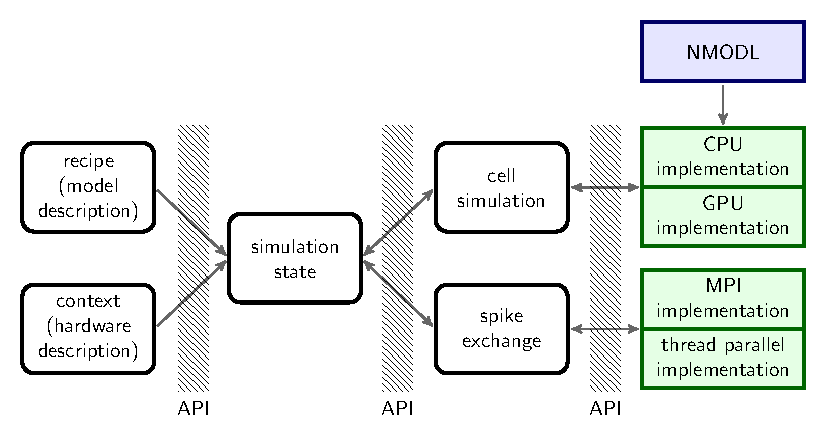
\includegraphics[width=0.8\textwidth]{images/api.pdf}
%    \end{center}
%    Adding a new hardware back end does not touch a single line of simulation state or front end code.
%\end{frame}
%-------------------------------------------

\cscschapter{2. Use flat descriptions in API.}

%-------------------------------------------
\begin{frame}[fragile]{}
    \emph{Observation}: constructing descriptions of single cells is the main portability
    challenge with multicompartment models developed for NEURON.

    \vspace{10pt}
    \begin{enumerate}
        \item \textcolor{green!50!black}{\ding{51}} The NMODL language describes dynamics of individual mechanisms.
        \item \textcolor{red}{\ding{55}} Distribution and properties of mechanisms are described with a Turing complete language
              like Python/HOC.
    \end{enumerate}
    \vspace{10pt}
    \emph{The challenge}: Models need to describe morphologies, and locations and regions on the morphology.
\end{frame}
%-------------------------------------------

%-------------------------------------------
\begin{frame}[fragile]{Step 1: Morphology Representation}
    Cells are composed of \emph{cable segments}:
    \begin{itemize}
        \item truncated conic frustums, not cylinders;
        \item we removed support for a spherical segment at ``soma''.
        %\item can be dislocated;
        %\item form branches (c.f. SONATA sections).
    \end{itemize}

    \begin{center}
        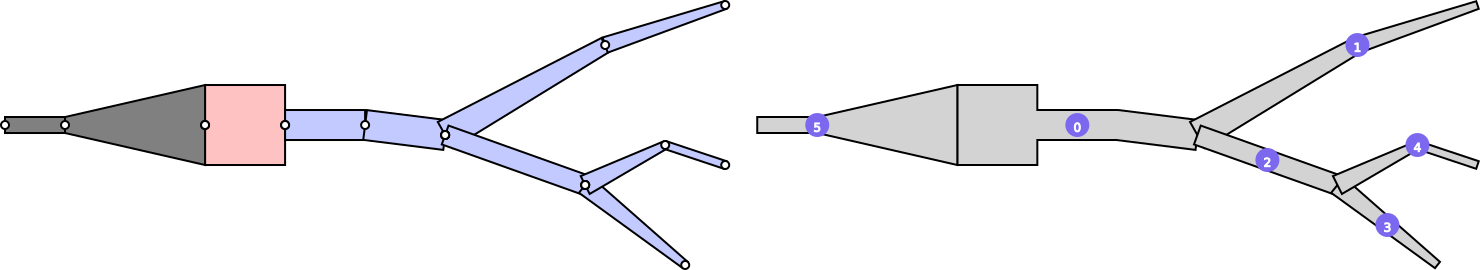
\includegraphics[width=\textwidth]{./morphos/morphlab.png}
        \\
        \small \textit{(Left) Segments (red=soma, grey=axon, blue=dend);\\(right) The branches.}
    \end{center}

    This can represent NeuroML, SWC and Neurolicida formats.
    \begin{itemize}
        \item \texttt{<rant>} \textit{please} don't use ``spherical'' somas in SWC files: it makes no sense. \texttt{</rant>}
    \end{itemize}

\end{frame}
%-------------------------------------------

%-------------------------------------------
\begin{frame}[fragile]{Step 2: Define regions and locations}

    A \emph{locset} is a multiset of locations on a morphology, e.g.:
    \begin{itemize}
        \item The center of the soma.
        \item The locations of inhibitory synapses.
        \item The tips of the dendritic arbor.
    \end{itemize}
    \vspace{5pt}

    A \emph{region} is a subset of a morphology's cable segments, e.g.:
    \begin{itemize}
        \item The soma.
        \item The dendritic arbor.
        \item Everywhere more distant than 100 $\mu$m from the soma.
        \item The dendrites with radius less than 1 $\mu$m.
    \end{itemize}
    \vspace{5pt}
    \arbor provides a DSL for their succinct description.

\end{frame}
%-------------------------------------------

%-------------------------------------------
\begin{frame}[fragile]{The region and locset DSL}
    The DSL uses \emph{s-expressions} and is composable:

    \begin{lstlisting}[style=arblang]
(distal_interval             ; take subtrees that start at
  (proximal                  ; locations closest to the soma
    (radius_lte              ; with radius <= 0.2 um
      (join (tag 3) (tag 4)) ; on basal and apical dendrites
      0.2)))
    \end{lstlisting}

    Expressions are given labels in a dictionary:

    \begin{lstlisting}[style=talkpython]
labels = {'soma': '(tag 1)',
          'axon': '(tag 2)',
          'dend': '(tag 3)',
          'apic': '(tag 4)',
          'inhib': '(uniform (region "dend")   0  99 0)',
          'stim': '(cable 0 0.5)'}
    \end{lstlisting}

    Replace \& simplify non-portable and bug-prone hoc templates.
    \begin{itemize}
        \item Describes what, not how.
        \item Not part of the morphology description.
    \end{itemize}

\end{frame}
%-------------------------------------------

%-------------------------------------------
\begin{frame}[fragile]{Region and locset examples}
    \begin{columns}[T]
        \begin{column}{0.5\textwidth}
            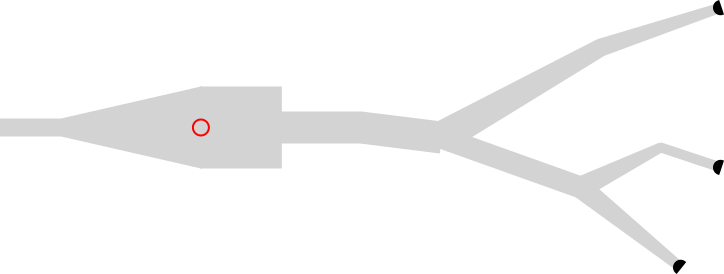
\includegraphics[width=\textwidth]{images/ls_term.png}

            \vspace{10pt}

            \begin{lstlisting}[style=arblang]
(restrict (terminal) (tag 3))
            \end{lstlisting}

            The tips (terminals) of the dendritic arbor (tag 3).

        \end{column}
        \begin{column}{0.5\textwidth}
            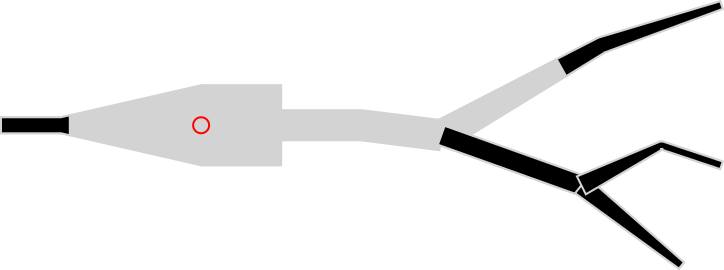
\includegraphics[width=\textwidth]{images/reg_radle5.png}

            \vspace{10pt}

            \begin{lstlisting}[style=arblang]
(radius_le (all) 0.5)
            \end{lstlisting}
            All parts of the cell with radius less than or equal to 0.5 $\mu$m.

        \end{column}
    \end{columns}
\end{frame}
%-------------------------------------------

%-------------------------------------------
\begin{frame}[fragile]{Step 3: Build a cell and decorate}

    \begin{lstlisting}[style=talkpython]
import arbor as arb

# Create a cable_cell description
labels = {...}
morph = arb.swc_import('purkinje.swc')
cell = arb.cable_cell(morph, labels)

# Bind mechanisms to regions and synapses to locsets
cell.paint('soma', 'hh')
cell.paint('dend', 'pas')
cell.paint('axon', 'pas/g=0.0012')
cell.place('inhib', 'expsyn')

# Attach spike detector and a current clamp
cell.place('(root)', arb.spike_detector(thresh=-10))
cell.place('stim',   arb.i_clamp(delay=10, duration=10, amplitude=0.4))
    \end{lstlisting}
\end{frame}
%-------------------------------------------

%-------------------------------------------
\begin{frame}[fragile]{A flat interface.}
    This interface requires three separate flat bits of information to define a single cell:

    \vspace{10pt}

    \begin{enumerate}
        \item A morphology description (e.g. an SWC file)
        \item A dictionary that maps labels to regions and locset definitions.
        \item A mapping of mechanisms and their properties to regions and locations.
    \end{enumerate}

    \vspace{10pt}

    \arbor provides composable policies for compartmentalization, or explicit compartmentalization, that is \textit{independent} of the model description.
\end{frame}
%-------------------------------------------

\cscschapter{Testing with the The Allen SDK}

%-------------------------------------------
\begin{frame}[fragile]{Allen SDK: models}
    The Allen SDK provides programatic access to a wide range of open data sets and models from the Allen Institute.

    \vspace{10pt}
    Single cell models are described with:
    \begin{enumerate}
        \item An SWC morphology.
        \item JSON file with mechanism and electrical properties with fitted parameters on regions.
        \item Electrophysiology measurements.
    \end{enumerate}
    \vspace{10pt}
    \emph{Aim}: write an \arbor wrapper for Allen SDK descriptions and validate againts \neuron.
\end{frame}
%-------------------------------------------
%-------------------------------------------
\begin{frame}[fragile]{Allen SDK: porting}
    The first 90\% was easy (about 2 days):
    \begin{itemize}
        \item half a day to install Allen SDK, \neuron and \arbor.
        \item half a day to update Allen NMODL files for \arbor.
        \item half a day to get the model running in each simulator.
    \end{itemize}
    \vfill

    The last 10\%, to get match results took longer (a week):
    \begin{itemize}
        \item Allen SDK modifies axon geometry to after loading.
        \item \neuron automatically enables usine the Nernst equation under certan circumstances.
        \item The JSON inputs are not fully uniform across all models.
        \item Spherical somas in SWC files are a bit magic.
    \end{itemize}
\end{frame}
%-------------------------------------------

%-------------------------------------------
\begin{frame}[fragile]{Allen SDK: results}
    \vfill
    Results from running the model with Python 3.8 on a 2018 Macbook:
    \begin{itemize}
        \item \neuron v7.7 (pip): 118s.
        \item \arbor v0.3.dev (cmake): 14s.
    \end{itemize}

    \vspace{-15pt}

    \begin{center}
    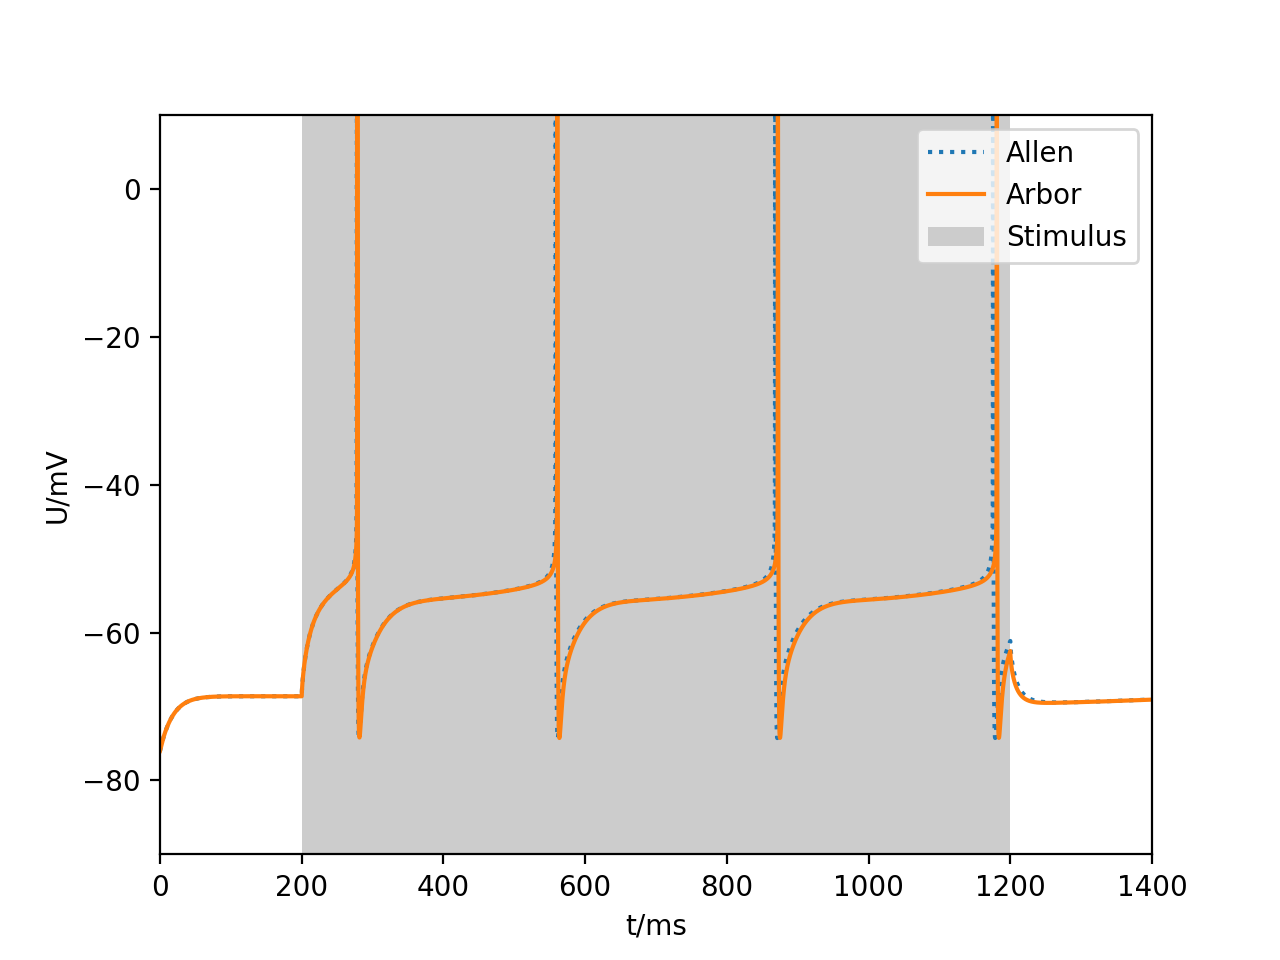
\includegraphics[width=0.75\textwidth]{images/allen-vs-arbor-no-sphere-here.png}
    \end{center}

\end{frame}
%-------------------------------------------

%-------------------------------------------
\begin{frame}[fragile]{Allen SDK: conclusion}
    The Allen SDK single cell model descriptions do a good job of separating model description from the simulation tool.

    \vspace{20pt}

    It isn't perfect, however the issues are all simple to address.

    \vspace{20pt}

    There are no significant barriers to using \arbor in The Allen SDK.
\end{frame}
%-------------------------------------------

%-------------------------------------------
%\begin{frame}[fragile]{Retrospective}
    %After 5 years of development we have come to realise that...
    %\begin{itemize}
        %\item The number one road block stopping adoption of new tools is non-portable model descitions.
        %\item Time spent hacking on low level GPU/CPU code is much less than the time spent on interfaces.
    %\end{itemize}
    %\vspace{10pt}
    %SONATA is a promising move towards portability.
%\end{frame}
%-------------------------------------------

%-------------------------------------------
\begin{frame}[fragile]{The end}
    \arbor is under active, open, development.

    \vspace{10pt}

    \begin{center}
        \arbor is \emph{open source software}:\\
        \vspace{3pt}
        \begin{lstlisting}[style=talkpseudo]
                  github.com/arbor-sim/arbor
        \end{lstlisting}
    \end{center}

    Version 0.4 with full support for Allen SDK mechanisms and morphology descriptions will be released very soon.
\end{frame}
%-------------------------------------------

%-------------------------------------------
\begin{frame}[fragile]{}
    \begin{center}
        
\includegraphics[height=0.15\textwidth]{logos/HBP_logo.jpg}
        \\ \vfill

        This research has received funding from the European Union’s Horizon 2020 Framework Programme for Research
        and Innovation under the Specific Grant Agreement No.  720270 (Human Brain Project SGA1), and Specific Grant
        Agreement No. 785907 (Human Brain Project SGA2).
        \\ \vfill

        
\includegraphics[height=0.1\textwidth]{logos/julich_logo.pdf}
        \hspace{1cm}
        
\includegraphics[height=0.09\textwidth]{logos/cscs_logo.pdf}
    \end{center}

\end{frame}
%-------------------------------------------


\end{document}
